% Beta-methylamino-DL-alanine - C4H10N2O2
% https://chemicalaid.com/tools/molarmass.php?formula=C4N2O2H10
% Coordinates found on https://tex.stackexchange.com/q/453740.

\documentclass[tikz]{standalone}

\pgfdeclarelayer{background}
\pgfsetlayers{background, main}

\begin{document}

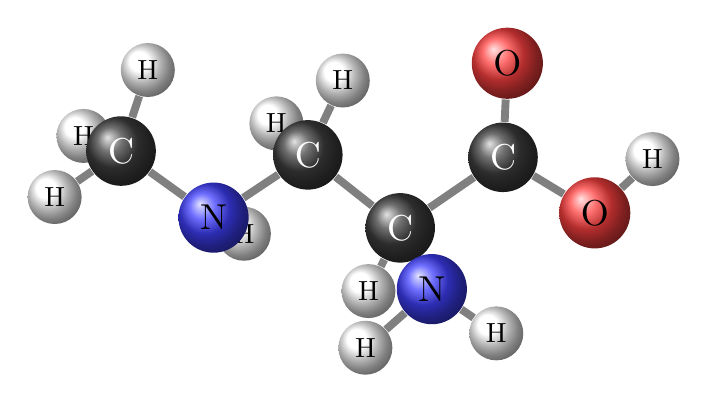
\begin{tikzpicture}
  \node[ball color=white, circle] (H1) at (-3.17, 1.39, -0.92) {H};
  \node[ball color=white, circle] (H2) at (-3.31, 1.23, 0.84) {H};
  \node[ball color=white, circle] (H3) at (-4.08, 0.05, -0.21) {H};
  \node[ball color=white, circle] (H4) at (-1.95, -0.69, -0.92) {H};
  \node[ball color=white, circle] (H5) at (-0.86, 1.39, 0.84) {H};
  \node[ball color=white, circle] (H6) at (-0.69, 1.26, -0.91) {H};
  \node[ball color=white, circle] (H7) at (0.46, -0.59, 1.23) {H};
  \node[ball color=white, circle] (H8) at (1.39, -1.82, -0.57) {H};
  \node[ball color=white, circle] (H9) at (-0.23, -1.96, -0.46) {H};
  \node[ball color=white, circle] (H10) at (3.57, 0.59, -0.06) {H};
  \node[ball color=black!75, circle, white, scale=1.3] (C1) at (-3.19, 0.68, -0.09) {C};
  \node[ball color=black!75, circle, white, scale=1.3] (C2) at (-0.78, 0.67, 0.01) {C};
  \node[ball color=black!75, circle, white, scale=1.3] (C3) at (0.47, -0.18, 0.21) {C};
  \node[ball color=black!75, circle, white, scale=1.3] (C4) at (1.73, 0.67, 0.09) {C};
  \node[ball color=blue!75, circle, scale=1.3] (N1) at (-2.00, -0.15, -0.05) {N};
  \node[ball color=blue!75, circle, scale=1.3] (N2) at (0.51, -1.32, -0.73) {N};
  \node[ball color=red!75, circle, scale=1.3] (O1) at (1.80, 1.88, 0.13) {O};
  \node[ball color=red!75, circle, scale=1.3] (O2) at (2.86, -0.07, 0.00) {O};
  \begin{pgfonlayer}{background}
    \draw[gray, line width=1mm] (H1) -- (C1) -- (N1) -- (C2) -- (C3) -- (C4) -- (O1) (H2) -- (C1) (H3) -- (C1) (N1) -- (H4) (C2) -- (H5) (C2) -- (H6) (C3) -- (H7) (C3) -- (N2) -- (H8) (N2) -- (H9) (C4) -- (O2) -- (H10);
  \end{pgfonlayer}
\end{tikzpicture}

\end{document}